\documentclass{IEEEtran}

\author{Piers R. Williams, \and Joseph Walton-Rivers}

\title{MCTS Applied to Co-operative Problems}

\usepackage{graphicx}
\usepackage{glossaries}

\newacronym{mcts}{MCTS}{Monte-Carlo Tree Search}
\newacronym{uct}{UCT}{Uniform Cost applied to Trees}
\newacronym{ggp}{GGP}{General Game Playing}
\newacronym{ga}{GA}{Genetic Algorithm}
\newacronym{mas}{MAS}{Multi-Agent Systems}

\begin{document}
\maketitle
\begin{abstract}
This paper highlights an experiment to see how standard \gls{mcts} handles simple co-operative problems.	These problems are formed from a simple grid world that has a set of goals, doors and buttons as well as walls that cannot be walked through. Two agents have to each reach every goal present on the map. For a door to be open, an Agent must be present on at least one of the buttons that is linked to it.

When laid out correctly, the world requires each agent to do certain things at certain times in order to achieve the goal. With no modification to allow communication between the two Agents - \gls{mcts} performs well and performs very 'purposefully' when given enough computational time.
\end{abstract}

\section{Introduction}

\gls{mcts} has been applied to a wealth of domains and is one of the primary algorithms in use for \gls{ggp}\cite{finnsson2008simulation}. Primary advantages are that, when given a sufficient forward model, \gls{mcts} doesn't require any knowledge about the game itself in order to play.

Standard \gls{mcts} plays best when it is either able to search to the end of the game tree, or is given rewards frequently. \gls{mcts} tends to stumble when the time given to it isn't sufficient to allow it to locate any sequence of actions that provides a reward in order to differentiate the root's children.

Traditional \gls{mas} would be the logical choice for solving this type of problem, however they were left out in order to work towards a co-operative \gls{ggp} agent.

Creating \gls{ggp} agents that can co-operate with other players would open the door for more flexible agents in games that can work together with human players. 
\section{The Experiment}
The main premise was to put \gls{mcts} in a situation where it would rely on other AI Agents in order to achieve its objectives, as well as provide a code base for further work with communication between Agents. In order to do this, a problem domain was created.
\subsection{The Problem Domain}
The problem domain is a simple grid world consisting of various objects:
\begin{itemize}
\item{\emph{Walls -} Walls are impassable, and are fixed in position. \emph{Doors} are rendered in Black.}
\item{\emph{Agents -} Agents are the moving objects that can activate buttons and the goal. \emph{Agents} are rendered in dark Yellow}
\item{\emph{Doors -} Doors are impassable, unless a linked \emph{Button} is currently activated. \emph{Doors} are rendered in Blue unless they are open}
\item{\emph{Buttons -} Buttons are passable, and when an \emph{Agent} is on the \emph{Button} it will activate and open the linked \emph{Door}. \emph{Buttons} are rendered in Red}
\item{\emph{Goals -} Goals are passable and reward all \emph{Agents} with a portion of the score. All \emph{Goals} are worth the same amount and the maximum score of $1$ is achieved when every \emph{Agent} has visited every \emph{Goal} at least once. Re-visiting a \emph{Goal} has no effect. \emph{Goals} are rendered in Yellow}
\end{itemize}

The starting positions for a simple problem is shown in Figure \ref{InitialState}
\begin{figure}[ht]
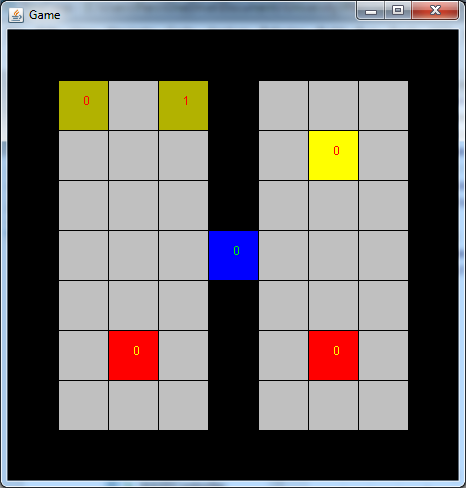
\includegraphics[scale=0.5]{InitialState}
\caption{Simple game state showing the different elements}
\label{InitialState}
\end{figure}

All levels are defined by a simple text file format.

The problems are designed to require Agents to co-operate in order to achieve their goals. Unlike other environments where \gls{mcts} can charge off achieving its own goals, this domain requires the agents to sometimes sit patiently on a button for another Agent to do something else.


\subsection{AI Controllers}
A small set of AI Controllers were created in order to attempt to solve the problem domain. None of the agents have the ability to communicate with another agent.
\subsubsection{Random}
The random controller simply chooses one of the possible 5 actions. This is one of the simplest to implement and run.
\subsubsection{Keyboard}
The keyboard controller takes input from the keyboard and translates that into a single Action. Once an action is polled, it is reset to the No Op action unless the keyboard is used again. 
\subsubsection{\gls{mcts}}
The \gls{mcts} controller is a simple implementation of \gls{uct} - with a fixed iteration, \gls{uct} Border and rollout border. No knowledge about the game is provided and the assumption is made that the other player will play randomly. The fixed rollout border makes a significant improvement in iterations per decision (On the machine from 1-3 to 500-600 in 40ms). This greatly improves the ability of \gls{mcts} to make informed decisions. The score at the end of a rollout is taken from the game state - so if \gls{mcts} doesn't see any player reach a goal, all branches will be equal.
\subsubsection{A*}
An intelligent agent was required that could provide comparison to how the MCTS is performing. A Star was selected and written to view the problem as selecting the shortest path of actions that would result in reaching the goals.
\subsubsection{Macro Action Genetic Algorithm}
The \gls{ga} algorithm was selected for its simplicity and had Macro Actions added in order to improve the forward search capability.
\subsubsection{Variable Macro Action Genetic Algorithm}

\subsection{Initial Testing}
Initially, observations were made to see how \gls{mcts} handled the problem. At first, with a small computational budget it seemed like \gls{mcts} would perform poorly, with near random movement seeming to emerge.

This changed, when an agent (Agent 1 say) got near a \emph{Button} or \emph{Door}. When Agent 1 reached an item like this - Agent 2 would seemingly gain some purpose and typically head for the other items. When Agent 1 got on the \emph{Button}, Agent 2 would head straight through the open \emph{Door} and to the \emph{Goal}. Behaviour would then typically go back towards a more random approach, unless the Agent 1 got near the \emph{Door} - typically causing Agent 2 to head more purposefully towards the \emph{Button} that would allow Agent 1 to reach the \emph{Goal}.

With this observation made - the computational budget was increased ten-fold, and the \gls{mcts} agents performed significantly better. Typical behaviour would be near optimal with significantly less random sections of movement. This can likely be attributed to the increased rollout and uct border depths allowing more foresight on such a small puzzle.
\subsection{Tournament}
A round robin tournament with three maps and the assembled Agents with various parameters was run - allowing each Agent to be paired with every other Agent (including itself) and play the game ten times per level.
\bibliographystyle{IEEEtran}
\bibliography{ceec}

\end{document}